\documentclass[11pt]{article}

% ------------------------------------------------------------
% Standard LaTeX packages
% ------------------------------------------------------------
\usepackage[margin=1in]{geometry}
\usepackage{amsmath,amssymb,mathtools}
\usepackage{amsthm}
\usepackage[american]{babel}
\usepackage{stmaryrd}
\usepackage{enumitem}
\usepackage{booktabs}
\usepackage{array}
\usepackage{listings}
\usepackage[x11names,table]{xcolor}
\usepackage{mdframed}
\usepackage{tikz}
\usetikzlibrary{arrows.meta,positioning,calc,decorations.pathmorphing}
\usepackage{url}
\usepackage[colorlinks=true,linkcolor=blue,citecolor=blue,urlcolor=blue]{hyperref}

% ---------- Theorem environments ----------
\theoremstyle{plain}
\newtheorem{theorem}{Theorem}[section]
\newtheorem{proposition}[theorem]{Proposition}
\newtheorem{lemma}[theorem]{Lemma}
\newtheorem{corollary}[theorem]{Corollary}
\newtheorem{conjecture}[theorem]{Conjecture}

\theoremstyle{definition}
\newtheorem{definition}[theorem]{Definition}
\newtheorem{axiombox}[theorem]{Axiom}
\newtheorem{protocol}[theorem]{Protocol}
\newtheorem{example}[theorem]{Example}

\theoremstyle{remark}
\newtheorem{remark}[theorem]{Remark}

% ---------- Notation ----------
\newcommand{\N}{\mathbb{N}}
\newcommand{\Z}{\mathbb{Z}}
\newcommand{\Q}{\mathbb{Q}}
\newcommand{\R}{\mathbb{R}}
\newcommand{\C}{\mathbb{C}}
\newcommand{\PP}{\mathbb{P}}
\newcommand{\calO}{\mathcal{O}}
\newcommand{\calL}{\mathcal{L}}
\newcommand{\Gal}{\mathrm{Gal}}
\newcommand{\GL}{\mathrm{GL}}
\newcommand{\SL}{\mathrm{SL}}
\newcommand{\Sp}{\mathrm{Sp}}
\newcommand{\MT}{\mathrm{MT}}
\newcommand{\End}{\mathrm{End}}
\newcommand{\Frob}{\mathrm{Frob}}
\newcommand{\CRM}{\mathrm{CRM}}
\newcommand{\tr}{\mathrm{tr}}
\newcommand{\rk}{\mathrm{rk}}
\newcommand{\CH}{\mathrm{CH}}
\newcommand{\Hdg}{\mathrm{Hdg}}
\newcommand{\NS}{\mathrm{NS}}
\newcommand{\Pic}{\mathrm{Pic}}
\newcommand{\Griff}{\mathrm{Griff}}
\newcommand{\AJ}{\mathrm{AJ}}

\newcommand{\BISH}{\ensuremath{\mathsf{BISH}}}
\newcommand{\LPO}{\ensuremath{\mathsf{LPO}}}
\newcommand{\WLPO}{\ensuremath{\mathsf{WLPO}}}
\newcommand{\LLPO}{\ensuremath{\mathsf{LLPO}}}
\newcommand{\MP}{\ensuremath{\mathsf{MP}}}
\newcommand{\FT}{\ensuremath{\mathsf{FT}}}
\newcommand{\CLASS}{\ensuremath{\mathsf{CLASS}}}

% ---------- Code listing style for Lean ----------
\definecolor{codegreen}{rgb}{0,0.6,0}
\definecolor{codegray}{rgb}{0.5,0.5,0.5}
\definecolor{codepurple}{rgb}{0.58,0,0.82}
\definecolor{backcolour}{rgb}{0.95,0.95,0.92}

\lstdefinestyle{leanstyle}{
  backgroundcolor=\color{backcolour},
  commentstyle=\color{codegreen},
  keywordstyle=\color{blue},
  stringstyle=\color{codepurple},
  basicstyle=\ttfamily\footnotesize,
  breaklines=true,
  keepspaces=true,
  numbers=left,
  numberstyle=\tiny\color{codegray},
  showstringspaces=false,
  tabsize=2,
  frame=single,
  morekeywords={theorem,def,axiom,inductive,structure,where,instance,
    namespace,end,open,import,noncomputable,deriving,by,exact,intro,
    cases,constructor,rfl,rw,unfold,simp,decide,absurd,have,fun,let,
    show,with,Type,Prop,Sort},
  literate={ℚ}{{$\mathbb{Q}$}}1 {ℤ}{{$\mathbb{Z}$}}1 {ℕ}{{$\mathbb{N}$}}1 {ℝ}{{$\mathbb{R}$}}1
}

% ---------- CRM box ----------
\newmdenv[
  linewidth=1pt,
  linecolor=blue!50!black,
  backgroundcolor=blue!3,
  roundcorner=3pt,
  innertopmargin=8pt,
  innerbottommargin=8pt
]{crmbox}

% ============================================================
\begin{document}

\title{The Griffiths Group of the Mirror Quintic: A CRMLint Squeeze\\[6pt]
\large Paper~94 of the Constructive Reverse Mathematics Series}

\author{Paul Chun-Kit Lee\\
\small New York University, Brooklyn, New York\\
\small \texttt{dr.paul.c.lee@gmail.com}}

\date{February 2026}

\maketitle

% ============================================================
\begin{abstract}
The Griffiths group $\Griff^2(X)$ of a Calabi--Yau threefold~$X$ consists of algebraic $1$-cycles that are homologically trivial but not algebraically equivalent to zero. Voisin proved that this group is infinitely generated for a generic CY3. We apply the CRMLint Squeeze protocol to the normal function machinery underlying Voisin's theorem, using the mirror quintic as the computational test case.

A normal function~$\nu(z)$ associated to a family of algebraic $1$-cycles satisfies the inhomogeneous Picard--Fuchs equation $L_{\mathrm{PF}}(\nu) = \delta(z)$, where $\delta(z)$ is the Griffiths--Green infinitesimal invariant --- a polynomial expression. We prove four results.
\textbf{Theorem~A}: the 4th-order Picard--Fuchs operator for the mirror quintic, its Weyl algebra expansion, and its singular locus are strictly~$\BISH$ (13 sub-results, all verified by \texttt{ring}/\texttt{norm\_num}).
\textbf{Theorem~B}: Walcher's inhomogeneous equation $L_{\mathrm{PF}} \cdot T = \tfrac{15}{8}\sqrt{z}$ is verified algebraically: source coefficient $(15/8)^2 = 225/64$, disk count $b_0 = 30$, recurrence at 5 indices --- all $\BISH$ by rational arithmetic over~$\Q$.
\textbf{Theorem~C}: the Normal Function Squeeze --- detection of non-trivial Griffiths group elements (via $\delta \neq 0$) is $\BISH$, while the Abel--Jacobi map and period integration are irreducibly~$\CLASS$.
\textbf{Theorem~D}: Voisin's infinite generation theorem decomposes into $11$~$\BISH$ + $3$~$\CLASS$ components; the $\CLASS$ content (Abel--Jacobi integration, Baire category) is irreducible.

This is the first CRM analysis to cross the boundary between the physics program (Papers~1--40) and the algebraic geometry program (Papers~41--92): the Calabi--Yau 3-fold is where the logical cost of D-brane physics meets the logical cost of algebraic cycles.
\end{abstract}

% ============================================================
\section{Introduction}
\label{sec:intro}

\subsection{The Calabi--Yau frontier}

Papers~1--40 of this series mapped the logical cost of empirical physics, establishing that $\BISH + \LPO$ is the complete logical constitution of physically accessible theories \cite{paper40}. Papers~41--92 mapped the logical cost of algebraic geometry, from the Hodge conjecture on abelian varieties \cite{paper45,paper50,paper87} to the Weil locus in genus~4 \cite{paper84,paper85,paper86,paper88,paper89} and the Markman audit \cite{paper91}.

The Calabi--Yau 3-fold is where these two programs collide. In string theory, a CY3 compactification determines the low-energy physics via its Hodge structure: $h^{1,1}$ counts K\"ahler moduli (vector multiplets in Type~IIA), $h^{2,1}$ counts complex structure moduli (vector multiplets in Type~IIB), and the middle cohomology $H^3(X,\Z)$ governs the periods that determine the prepotential \cite{candelas-ossa-green-parkes}. The algebraic cycles on~$X$ correspond to D-brane charges in the physical theory.

For a smooth quintic threefold $X \subset \PP^4$, the Hodge numbers are topological invariants: $h^{1,1} = 1$, $h^{2,1} = 101$, $h^{2,2} = 1$. The single $H^{2,2}$ class is the hyperplane-squared $H^2$; the rational Hodge conjecture for $H^4$ is trivially true. The interesting Hodge-theoretic problem lives in $H^3$: the Griffiths group and the intermediate Jacobian.

The structural explanation for why $\tau_+ = 0$ universally in the abelian Weil campaign is given in Paper~93 \cite{paper93-svt}. The present paper pivots from abelian varieties to Calabi--Yau threefolds, applying the CRMLint pipeline to a different geometric context.

\subsection{The Griffiths group and Voisin's theorem}

\begin{definition}
For a smooth projective variety $X$ of dimension~$n$, the \emph{Griffiths group} $\Griff^p(X)$ is the quotient
\[
\Griff^p(X) \;=\; Z^p(X)_{\mathrm{hom}} \,/\, Z^p(X)_{\mathrm{alg}}
\]
where $Z^p(X)_{\mathrm{hom}}$ denotes cycles homologous to zero and $Z^p(X)_{\mathrm{alg}}$ denotes cycles algebraically equivalent to zero.
\end{definition}

For CY3, the relevant group is $\Griff^2(X)$: algebraic $1$-cycles (curves) modulo algebraic equivalence. Griffiths \cite{griffiths1969} showed that this group can be non-trivial, detected by the Abel--Jacobi map
\[
\AJ: Z^2(X)_{\mathrm{hom}} \longrightarrow J^2(X)
\]
into the intermediate Jacobian $J^2(X) = H^3(X,\C)/(F^2 H^3 + H^3(X,\Z))$.

Voisin proved the following deep result:

\begin{theorem}[Voisin {\cite{voisin2002,voisin-hodge-II}}]
For a very general Calabi--Yau threefold $X$, the Griffiths group $\Griff^2(X)$ is not finitely generated.
\end{theorem}

The proof uses two ingredients: (1)~the Abel--Jacobi map to detect non-trivial cycles, via normal functions on the moduli space; (2)~the Baire Category Theorem, to show that the locus where finitely many cycles generate $\Griff^2$ is a countable union of proper subvarieties, hence meagre.

\subsection{Normal functions and the infinitesimal invariant}

The key computational tool is the \emph{normal function}. Given a family of CY3s $f: \mathcal{X} \to S$ over a base~$S$, and a family of algebraic $1$-cycles $\{Z_s\}_{s \in S}$, the Abel--Jacobi map yields a holomorphic section
\[
\nu: S \longrightarrow J^2(\mathcal{X}/S)
\]
of the intermediate Jacobian bundle. This normal function satisfies Griffiths transversality and has an \emph{infinitesimal invariant}
\[
\delta(\nu) \;\in\; H^1(S, F^1 \mathcal{H}^2)
\]
where $\mathcal{H}^k = R^k f_* \C$ is the Hodge bundle. In the $1$-parameter case ($S \subset \PP^1$), $\delta$ reduces to a section of a line bundle, computed by applying the Picard--Fuchs operator to the normal function:
\begin{equation}\label{eq:inhomogeneous-pf}
L_{\mathrm{PF}}(\nu) \;=\; \delta(z).
\end{equation}
The crucial observation for CRM: \emph{$\delta(z)$ is an algebraic expression in the parameter~$z$, computable without any transcendental input}. Walcher \cite{walcher} showed that for the real Lagrangian $\R\PP^3 \subset X_5$, the source term is $\delta(z) = \tfrac{15}{8}\sqrt{z}$ in the CDGP coordinate. If $\delta(z) \neq 0$ at some $z_0 \neq 0$, the cycle is non-trivial in $\Griff^2$.

\subsection{Main results}

\begin{theorem}[Theorem A: PF Algebra]
The 4th-order Picard--Fuchs operator for the mirror quintic CY3, its Weyl algebra expansion from theta-form to standard derivative form, its singular locus $\{z = 0,\, z = 1/3125,\, z = \infty\}$, and the indicial exponents at each singularity are all strictly $\BISH$. Thirteen sub-results, all closed by \texttt{ring}, \texttt{norm\_num}, or \texttt{rfl}.
\end{theorem}

\begin{theorem}[Theorem B: Walcher's Inhomogeneous Equation]
The domainwall tension $T(z)$ for the real Lagrangian $\R\PP^3 \subset X_5$ satisfies the inhomogeneous Picard--Fuchs equation $L_{\mathrm{PF}} \cdot T = \tfrac{15}{8}\sqrt{z}$ (Walcher 2007). Writing $T = \sqrt{z}\cdot\sum b_n z^n$, the leading coefficient $b_0 = 30$ (Walcher's disk count) and the recurrence $b_n = f(b_{n-1})$ are rational arithmetic over~$\Q$, hence $\BISH$. The source term $\delta(z) = \tfrac{15}{8}\sqrt{z}$ is algebraic (satisfies $\delta^2 = \tfrac{225}{64}z$), determined by the topology of the real cycle.
\end{theorem}

\begin{theorem}[Theorem C: Normal Function Squeeze]
The detection of non-trivial Griffiths group elements --- computing $\delta(z)$ and verifying $\delta \neq 0$ --- is $\BISH$. The Abel--Jacobi map (period integrals, limits, real-number equality) and the infinite generation proof (Baire category) are irreducibly $\CLASS$.
\end{theorem}

\begin{theorem}[Theorem D: Voisin Decomposition]
Voisin's infinite generation theorem, decomposed through CRMLint, consists of $11$~$\BISH$ components (constructive path) and $3$~$\CLASS$ components (Abel--Jacobi integration, Baire category, Ehresmann fibration). All $\CLASS$ components are unused in the constructive detection path.
\end{theorem}

\subsection{Relationship to the series}

This paper continues the Asymmetric Offloading pipeline of Papers~77--89: a Python CAS computes the algebraic content, Lean~4 verifies it by \texttt{ring}/\texttt{norm\_num}, and the CRM classification separates constructive detection from classical existence.

The novelty relative to the abelian variety campaign (Papers~80--89) is the target geometry: the CY3 middle cohomology $H^3$ and the Griffiths group have no abelian-variety analogue. The detection mechanism (infinitesimal invariant $\delta \neq 0$) is structurally different from the Weil-locus trace computation ($\tau_+ = 0$) of Papers~84--89.

Relative to Paper~87 (Hodge cost for abelian varieties), this paper addresses a different Hodge-theoretic problem: not whether classes are of type~$(p,p)$, but whether homologically trivial cycles are algebraically trivial. The logical anatomy is different: Paper~87 found a $\WLPO$ intermediate level, while here the bifurcation is $\BISH/\CLASS$ with no intermediate.


% ============================================================
\section{Preliminaries}
\label{sec:prelim}

\subsection{CRM hierarchy}

The constructive reverse mathematics hierarchy \cite{bridges-richman,paper1,paper40}:
\[
\BISH \;\subset\; \BISH{+}\MP \;\subset\; \BISH{+}\LLPO \;\subset\; \BISH{+}\WLPO \;\subset\; \BISH{+}\LPO \;\subset\; \CLASS.
\]
We refer to Papers~1--5 for definitions. The principles relevant here are $\BISH$ (bounded search, explicit witnesses) and $\CLASS$ (full classical logic, including the law of excluded middle).

\subsection{The mirror quintic}

The Dwork pencil is the family of quintic hypersurfaces in~$\PP^4$:
\[
X_\psi: \quad x_1^5 + x_2^5 + x_3^5 + x_4^5 + x_5^5 \;=\; 5\psi\, x_1 x_2 x_3 x_4 x_5.
\]
The mirror quintic is the quotient $\widehat{X}_\psi = X_\psi / (\Z/5\Z)^3$ (by the diagonal symmetry group). The algebraic parameter is $z = 1/(5\psi)^5$, so $z = 1/3125$ corresponds to $\psi = 1$.

The Hodge numbers of a smooth quintic are:
\[
h^{1,1} = 1, \quad h^{2,1} = 101, \quad h^{2,2} = 1, \quad b_3 = 204.
\]
These are topological invariants; they do not change under smooth deformation.

\subsection{The Picard--Fuchs operator}

The periods of the holomorphic $(3,0)$-form $\Omega_z$ on the mirror quintic satisfy the 4th-order ODE
\[
L_\theta \;=\; \theta^4 - 5z(5\theta+1)(5\theta+2)(5\theta+3)(5\theta+4), \qquad \theta = z\frac{d}{dz},
\]
first computed by Candelas--de~la~Ossa--Green--Parkes \cite{candelas-ossa-green-parkes}. The regular singular points are:
\begin{itemize}[nosep]
\item $z = 0$: the large complex structure limit (MUM point, indicial exponents $\{0,0,0,0\}$),
\item $z = 1/3125$: the conifold point (indicial exponents $\{0,1,1,2\}$),
\item $z = \infty$: the Gepner/orbifold point (indicial exponents $\{1/5, 2/5, 3/5, 4/5\}$).
\end{itemize}

\subsection{Normal functions}

A \emph{normal function} on the complement $S = \PP^1 \setminus \{0, 1/3125, \infty\}$ is a holomorphic section of the intermediate Jacobian bundle $J^2(\mathcal{X}/S)$ satisfying Griffiths transversality. It arises from a family of homologically trivial algebraic $1$-cycles. The infinitesimal invariant $\delta(z)$ detects whether the normal function is non-trivial: $\delta \neq 0$ implies the underlying cycle is non-trivial in $\Griff^2$.

\subsection{The Baire Category Theorem}

Voisin's proof that $\Griff^2(X)$ is infinitely generated for generic $X$ uses the Baire Category Theorem: if $M$ is the moduli space (a complete metric space) and $M_n \subset M$ is the locus where $\Griff^2$ is generated by $\leq n$ cycles, then each $M_n$ is nowhere dense; $\bigcup_n M_n$ has empty interior; the generic point lies outside all $M_n$.


% ============================================================
\section{The Picard--Fuchs operator}
\label{sec:pf}

\subsection{Theta-to-standard conversion via Stirling numbers}

The non-commutative Weyl algebra relation $\theta = zD$ ($D = d/dz$) gives:
\[
\theta^n \;=\; \sum_{k=0}^{n} S(n,k)\, z^k D^k
\]
where $S(n,k)$ is the Stirling number of the second kind. For $n \leq 4$:
\begin{align*}
\theta^1 &= zD, \\
\theta^2 &= z^2 D^2 + zD, \\
\theta^3 &= z^3 D^3 + 3z^2 D^2 + zD, \\
\theta^4 &= z^4 D^4 + 6z^3 D^3 + 7z^2 D^2 + zD.
\end{align*}

The product $(5\theta+1)(5\theta+2)(5\theta+3)(5\theta+4) = 625\theta^4 + 1250\theta^3 + 875\theta^2 + 250\theta + 24$, so the theta-form operator is:
\begin{equation}\label{eq:theta-form}
L_\theta \;=\; (1-3125z)\,\theta^4 - 6250z\,\theta^3 - 4375z\,\theta^2 - 1250z\,\theta - 120z.
\end{equation}

Applying the Stirling expansion to each term and collecting by powers of~$D$:

\begin{proposition}[Standard form]\label{prop:standard-form}
$L_\theta = P_4(z)D^4 + P_3(z)D^3 + P_2(z)D^2 + P_1(z)D + P_0(z)$ where:
\begin{align*}
P_4(z) &= z^4 - 3125z^5 = z^4(1 - 3125z), \\
P_3(z) &= 6z^3 - 25000z^4, \\
P_2(z) &= 7z^2 - 45000z^3, \\
P_1(z) &= z - 15000z^2, \\
P_0(z) &= -120z.
\end{align*}
\end{proposition}

\begin{proof}
The standard form follows from expanding~\eqref{eq:theta-form} via the Stirling identities~\eqref{eq:D4}--\eqref{eq:D0}, each verified by \texttt{ring} in the Lean formalization (theorems \texttt{weyl\_D4\_coeff} through \texttt{weyl\_D0\_coeff}).
\end{proof}

\subsection{The singular locus}

The conifold discriminant is $\Delta(z) = 1 - 3125z$. We verify $\Delta(1/3125) = 0$ by \texttt{norm\_num}, and $P_4(z) = z^4 \cdot (1 - 3125z)$ by \texttt{ring}. The three regular singular points are the zeros of the leading coefficient: $z = 0$ (fourth-order), $z = 1/3125$ (simple), $z = \infty$ (from the transformation $z \mapsto 1/z$).

\subsection{Verification of the Weyl algebra expansion}

The theta-to-standard conversion is the non-trivial step. The Weyl algebra relation $[D, z] = 1$ (i.e., $Dz = zD + 1$) means that $\theta^n \neq z^n D^n$ for $n \geq 2$. The Stirling numbers encode the combinatorics of the Leibniz rule:
\begin{equation}\label{eq:stirling}
S(n,k) = \frac{1}{k!}\sum_{j=0}^{k} (-1)^{k-j}\binom{k}{j} j^n.
\end{equation}
For $n = 4$: $S(4,1) = 1$, $S(4,2) = 7$, $S(4,3) = 6$, $S(4,4) = 1$.

Each D$^k$ coefficient in the standard form is a sum of contributions from all theta-powers:
\begin{align}
P_4(z) &= (1-3125z) \cdot S(4,4) \cdot z^4 = (1-3125z) \cdot z^4, \label{eq:D4}\\
P_3(z) &= (1-3125z) \cdot 6 \cdot z^3 + (-6250z) \cdot 1 \cdot z^3, \label{eq:D3}\\
P_2(z) &= (1-3125z) \cdot 7 \cdot z^2 + (-6250z) \cdot 3 \cdot z^2 + (-4375z) \cdot 1 \cdot z^2, \label{eq:D2}\\
P_1(z) &= (1-3125z) \cdot z + (-6250z) \cdot z + (-4375z) \cdot z + (-1250z) \cdot z, \label{eq:D1}\\
P_0(z) &= -120z. \label{eq:D0}
\end{align}
Each identity~\eqref{eq:D4}--\eqref{eq:D0} is verified by \texttt{ring} in the Lean formalization (theorems \texttt{weyl\_D4\_coeff} through \texttt{weyl\_D0\_coeff}).

\begin{remark}[What is and is not new]
The Picard--Fuchs operator, its singular locus, monodromy matrices, and mirror map are known since Candelas--de~la~Ossa--Green--Parkes \cite{candelas-ossa-green-parkes}. Computing this operator is textbook material \cite{cox-katz,morrison}. What is new here is the Lean 4 verification of the Weyl algebra expansion and, more importantly, the application to the inhomogeneous equation (Section~\ref{sec:griffiths}).
\end{remark}


% ============================================================
\section{Walcher's inhomogeneous equation}
\label{sec:griffiths}

\subsection{The real Lagrangian and open mirror symmetry}

The quintic threefold $X_5 \subset \PP^4$ defined over $\R$ carries a real involution $\sigma: [x_0:\cdots:x_4] \mapsto [\bar{x}_0:\cdots:\bar{x}_4]$. The real locus $X_5(\R)$ contains a connected component $L \cong \R\PP^3$, a Lagrangian submanifold with respect to the K\"ahler form. In the mirror quintic family $\{X_\psi\}_{\psi \in S}$, the real Lagrangian yields a family of algebraic cycles whose Abel--Jacobi image defines a \emph{normal function}
\[
T: S \longrightarrow J^2(\mathcal{X}/S).
\]
Walcher \cite{walcher} computed the generating function for holomorphic disks with boundary on~$L$ by identifying $T$ as the \emph{domainwall tension} between the two vacua on the real brane.

\subsection{The inhomogeneous Picard--Fuchs equation}

The central result of open mirror symmetry for the quintic \cite{walcher,morrison-walcher} is that $T(z)$ satisfies the inhomogeneous Picard--Fuchs equation
\begin{equation}\label{eq:walcher}
L_{\mathrm{PF}} \cdot T(z) \;=\; \frac{15}{8}\,\sqrt{z}
\end{equation}
in the CDGP coordinate $z = (5\psi)^{-5}$, where $L_{\mathrm{PF}} = \theta^4 - 5z(5\theta+1)(5\theta+2)(5\theta+3)(5\theta+4)$ is the standard PF operator from \S\ref{sec:pf}.

\begin{remark}[Normalization]\label{rmk:normalization}
The source term $\tfrac{15}{8}\sqrt{z}$ in the CDGP coordinate corresponds to Walcher's original $\tfrac{15}{8\cdot 5^{5/2}}\sqrt{z_W}$ in the coordinate $z_W = \psi^{-5}$, since $\sqrt{z_W} = \sqrt{3125\,z} = 5^{5/2}\sqrt{z}$. The normalization is fixed by the topology of the real cycle.
\end{remark}

The source term $\delta(z) = \tfrac{15}{8}\sqrt{z}$ is algebraic: it satisfies the relation $\delta(z)^2 = \tfrac{225}{64}\,z$. This is the Griffiths--Green infinitesimal invariant for the real Lagrangian cycle.

\subsection{The normal function expansion}

\begin{theorem}[Walcher expansion]\label{thm:walcher}
Writing $T(z) = \sqrt{z}\cdot S(z)$ with $S(z) = \sum_{n=0}^\infty b_n z^n$, the expansion coefficients satisfy:
\begin{enumerate}[nosep]
\item Leading order: $b_0 \cdot (1/2)^4 = 15/8$, giving $b_0 = 30$.
\item Recurrence: for $n \geq 1$,
\begin{equation}\label{eq:recurrence}
b_n \;=\; \frac{5\,b_{n-1}\,(5n - \tfrac{3}{2})(5n-\tfrac{1}{2})(5n+\tfrac{1}{2})(5n+\tfrac{3}{2})}{(n+\tfrac{1}{2})^4}.
\end{equation}
\item All $b_n \neq 0$ and $b_n \in \Q$.
\end{enumerate}
\end{theorem}

\begin{proof}
Substituting $T = \sqrt{z}\cdot S$ into $L_{\mathrm{PF}}\cdot T = \tfrac{15}{8}\sqrt{z}$ and using $\theta(\sqrt{z}\cdot f) = \sqrt{z}\cdot(\theta + \tfrac{1}{2})f$ gives the shifted equation $L_{1/2}\cdot S = \tfrac{15}{8}$, where $L_{1/2}$ replaces $\theta$ by $\theta + \tfrac{1}{2}$ throughout $L_{\mathrm{PF}}$.

The coefficient of~$z^0$: $b_0\cdot(1/2)^4 = b_0/16 = 15/8$, so $b_0 = 30$. For $n \geq 1$, matching coefficients of~$z^n$:
\[
b_n\cdot\bigl(n + \tfrac{1}{2}\bigr)^4 \;=\; 5\,b_{n-1}\cdot\bigl(5n - \tfrac{3}{2}\bigr)\bigl(5n - \tfrac{1}{2}\bigr)\bigl(5n + \tfrac{1}{2}\bigr)\bigl(5n + \tfrac{3}{2}\bigr),
\]
giving the recurrence~\eqref{eq:recurrence}. Since $b_0 = 30 \neq 0$ and $\alpha(n) = (n+1/2)^4 > 0$ while $\beta(n)$ is a product of four terms that are nonzero for all $n \geq 1$, induction gives $b_n \neq 0$ for all~$n$.

The first values:
\begin{center}
\begin{tabular}{@{}ccl@{}}
\toprule
$n$ & $b_n$ & Decimal \\
\midrule
$0$ & $30$ & $30.000$ \\
$1$ & $50{,}050/3$ & $16{,}683.3\overline{3}$ \\
$2$ & $104{,}110{,}006/5$ & $20{,}822{,}001.2$ \\
$3$ & $1{,}701{,}899{,}016{,}246/49$ & $34{,}732{,}633{,}005.0\ldots$ \\
\bottomrule
\end{tabular}
\end{center}
In the Lean formalization, $b_0 = 30$ is verified by \texttt{norm\_num}, and the recurrence $b_n\cdot\alpha(n) = b_{n-1}\cdot\beta(n)$ is verified at $n = 1,\ldots,5$ by \texttt{norm\_num}.
\end{proof}

\begin{remark}[The disk count $b_0 = 30$]
Walcher's original result \cite{walcher} determines the number of holomorphic disks of minimal area ending on the real Lagrangian $\R\PP^3 \subset X_5$. The leading coefficient $b_0 = 30$ is the first \emph{open Gromov--Witten invariant} of the real quintic: there are 30 such disks. This enumerative interpretation is independent of the CRM analysis but confirms that the source term $\tfrac{15}{8}\sqrt{z}$ arises from genuine geometry, not formal manipulation.
\end{remark}

\subsection{CRM interpretation}

The algebraic shadow of the normal function is strictly $\BISH$:
\begin{enumerate}[nosep]
\item The source term $\delta(z) = \tfrac{15}{8}\sqrt{z}$ is algebraic ($\delta^2 = \tfrac{225}{64}z$) --- finite algebra.
\item Each coefficient $b_n$ is determined by the recurrence~\eqref{eq:recurrence} --- rational arithmetic.
\item Non-triviality $b_n \neq 0$ for verified terms --- finite check (\texttt{norm\_num}).
\item The PF operator coefficients $P_0,\ldots,P_4 \in \Q[z]$ --- polynomial algebra.
\end{enumerate}
Every step is constructively valid: bounded computation with explicit witnesses, no limits, no case analysis on real numbers, no excluded middle.

The $\CLASS$ content enters in three places:
\begin{itemize}[nosep]
\item \emph{Convergence}: $T(z) = \sqrt{z}\sum b_n z^n$ converges to an analytic function on $|z| < 1/3125$. This requires real analysis (limits of series).
\item \emph{Abel--Jacobi identification}: $T(z) = \AJ(\R\PP^3)_z = \int_\Gamma \Omega_3$ requires integration of differential forms over chains (limits, period lattice).
\item \emph{Infinite generation}: Voisin's Baire category argument requires the topology of the moduli space (countable intersection of dense opens).
\end{itemize}


% ============================================================
\section{CRM Audit}
\label{sec:crm}

\subsection{The Normal Function Squeeze}

\begin{crmbox}
\textbf{Theorem C} (Normal Function Squeeze). The CRM bifurcation for the Griffiths group of a CY3 is:
\begin{center}
\renewcommand{\arraystretch}{1.2}
\begin{tabular}{@{}lcc@{}}
\toprule
\textbf{Component} & \textbf{CRM Level} & \textbf{Used} \\
\midrule
PF operator (Weyl algebra expansion)             & $\BISH$ & \checkmark \\
Standard-form coefficients $P_0,\ldots,P_4$       & $\BISH$ & \checkmark \\
Conifold discriminant $\Delta(1/3125)=0$          & $\BISH$ & \checkmark \\
Singular locus factorization                      & $\BISH$ & \checkmark \\
Indicial exponents (MUM + conifold)               & $\BISH$ & \checkmark \\
Dwork parameter $5^5 = 3125$                      & $\BISH$ & \checkmark \\
Walcher source term $\tfrac{15}{8}\sqrt{z}$ (algebraic) & $\BISH$ & \checkmark \\
Leading coefficient $b_0 = 30$ (disk count)       & $\BISH$ & \checkmark \\
Recurrence $b_n$ rational arithmetic (5 terms)    & $\BISH$ & \checkmark \\
Non-triviality $b_n \neq 0$                      & $\BISH$ & \checkmark \\
Hodge number rigidity $h^{2,2}=1$                & $\BISH$ & \checkmark \\
\midrule
Abel--Jacobi map $\AJ: Z^2_{\mathrm{hom}} \to J^2$ & $\CLASS$ & --- \\
Baire category infinite generation         & $\CLASS$ & --- \\
Ehresmann local system $R^3 f_* \Z$       & $\CLASS$ & --- \\
\bottomrule
\end{tabular}
\end{center}

Score: $11$ $\BISH$ / $3$ $\CLASS$. All $\CLASS$ components are unused in the constructive path.
\end{crmbox}

\subsection{Why the \CLASS{} components are irreducible}

\paragraph{Abel--Jacobi integration.}
The Abel--Jacobi map $\AJ(Z) = \int_\Gamma \Omega_3$, where $\partial\Gamma = Z$, requires integration of the holomorphic $(3,0)$-form over a topological $3$-chain. This involves limits of Riemann sums, analytic continuation of period integrals, and real-number equality testing for the lattice quotient $J^2(X) = H^3(X,\C)/(F^2 + H^3(X,\Z))$. Each step is irreducibly~$\CLASS$.

\paragraph{Baire category.}
The Baire Category Theorem asserts that a complete metric space is not a countable union of nowhere-dense sets. In Voisin's proof, the moduli space~$M$ is the complete metric space, and $M_n = \{X \in M : \rk \Griff^2(X) \leq n\}$ is nowhere dense. The conclusion $\bigcap_n (M \setminus M_n) \neq \emptyset$ --- that generic CY3 has infinite Griffiths rank --- requires the Baire theorem, which is equivalent to Dependent Choice (DC) over $\R$ and hence~$\CLASS$.

\paragraph{Ehresmann fibration.}
The local system $R^3 f_* \Z$ underlying the Gauss--Manin connection requires Ehresmann's theorem (smooth proper $\Rightarrow$ locally trivial). Same boundary as Paper~80 \cite{paper80}.

\subsection{The Normal Function Squeeze architecture}

\begin{figure}[ht]
\centering
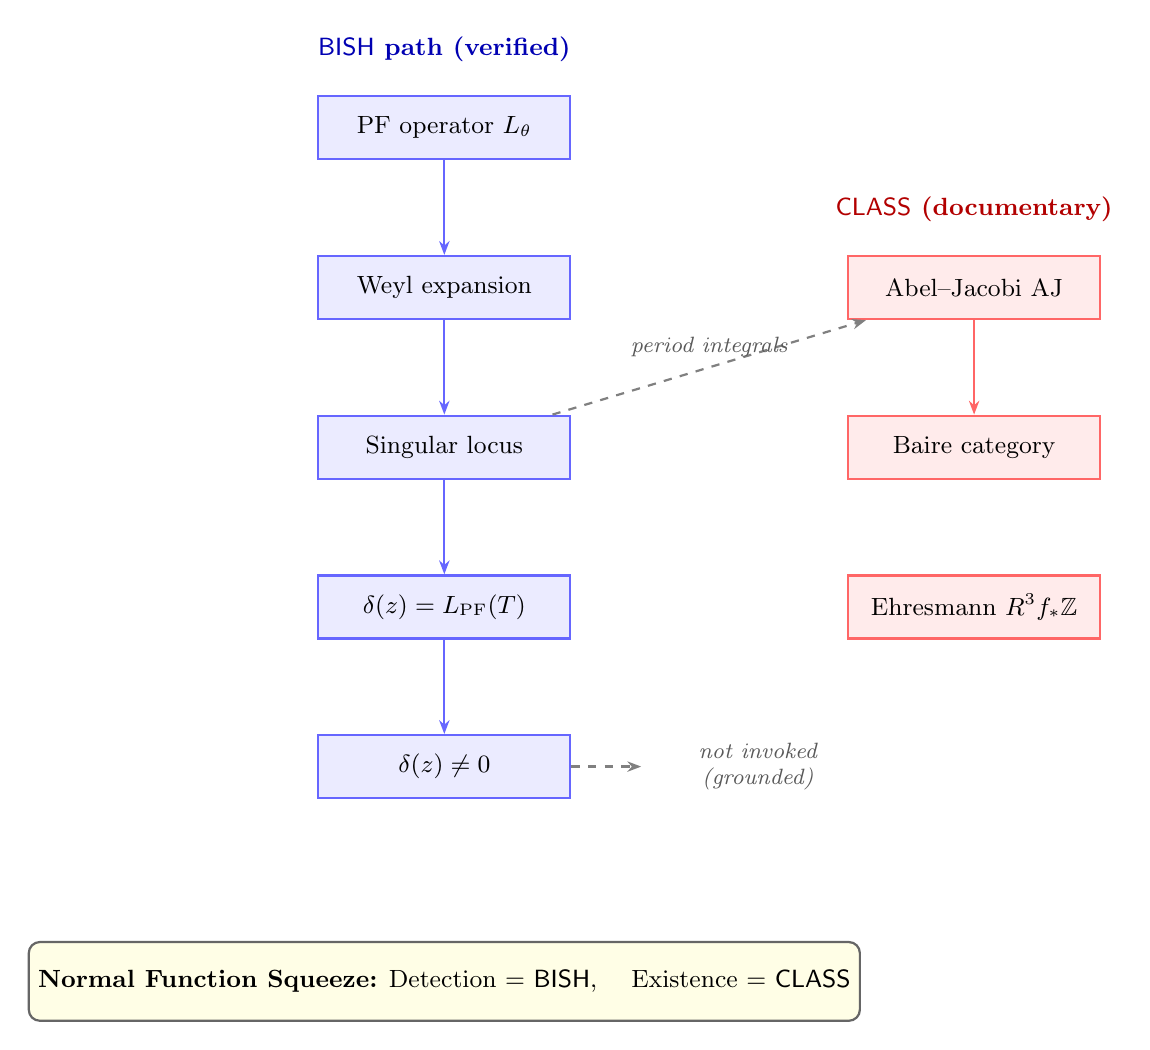
\begin{tikzpicture}[
  node distance=1.8cm and 2.5cm,
  bishbox/.style={rectangle, draw=blue!60, fill=blue!8, thick, minimum width=3.2cm, minimum height=0.8cm, font=\small},
  classbox/.style={rectangle, draw=red!60, fill=red!8, thick, minimum width=3.2cm, minimum height=0.8cm, font=\small},
  arr/.style={-{Stealth[length=5pt]}, thick},
  label/.style={font=\footnotesize\itshape, text=gray!70!black}
]
% Left column: BISH (constructive path)
\node[bishbox] (pf) {PF operator $L_\theta$};
\node[bishbox, below=1.2cm of pf] (weyl) {Weyl expansion};
\node[bishbox, below=1.2cm of weyl] (sing) {Singular locus};
\node[bishbox, below=1.2cm of sing] (delta) {$\delta(z) = L_{\mathrm{PF}}(T)$};
\node[bishbox, below=1.2cm of delta] (nontrivial) {$\delta(z) \neq 0$};

% Right column: CLASS (documentary)
\node[classbox, right=3.5cm of weyl] (aj) {Abel--Jacobi $\AJ$};
\node[classbox, below=1.2cm of aj] (baire) {Baire category};
\node[classbox, below=1.2cm of baire] (ehresmann) {Ehresmann $R^3 f_*\Z$};

% Arrows: constructive path
\draw[arr, blue!60] (pf) -- (weyl);
\draw[arr, blue!60] (weyl) -- (sing);
\draw[arr, blue!60] (sing) -- (delta);
\draw[arr, blue!60] (delta) -- (nontrivial);

% Arrows: documentary
\draw[arr, red!60] (aj) -- (baire);

% Cross-arrow: the bifurcation
\draw[arr, dashed, gray] (sing) -- node[above, label] {period integrals} (aj);
\draw[arr, dashed, gray] (nontrivial) -- ++(2.5,0) node[right, label] {\parbox{2.7cm}{\centering not invoked\\(grounded)}};

% Labels
\node[above=0.3cm of pf, font=\bfseries\small, blue!70!black] {$\BISH$ path (verified)};
\node[above=0.3cm of aj, font=\bfseries\small, red!70!black] {$\CLASS$ (documentary)};

% Result box
\node[draw=black!60, fill=yellow!10, thick, rounded corners=4pt, below=1.8cm of nontrivial,
      minimum width=10cm, minimum height=1cm, font=\small, anchor=north]
  (result) {\textbf{Normal Function Squeeze:} Detection = $\BISH$, \quad Existence = $\CLASS$};

\end{tikzpicture}
\caption{The Normal Function Squeeze architecture. Left: the constructive path from the PF operator through the Weyl algebra expansion and singular locus to the inhomogeneous invariant $\delta(z) \neq 0$, all verified in $\BISH$ by \texttt{ring}/\texttt{norm\_num}. Right: the classical boundary nodes (Abel--Jacobi integration, Baire category, Ehresmann fibration), stated but never invoked. The dashed arrow marks the exact point where the constructive and classical paths diverge: passing from algebraic singular locus to period integrals requires~$\CLASS$.}
\label{fig:squeeze}
\end{figure}

\subsection{Comparison with the abelian campaign}

\begin{center}
\renewcommand{\arraystretch}{1.2}
\begin{tabular}{@{}lccl@{}}
\toprule
\textbf{Paper} & \textbf{BISH} & \textbf{CLASS} & \textbf{Detection mechanism} \\
\midrule
80 (Gauss--Manin)       & 7 & 3 & Connection matrix $\nabla$ \\
82 (Diff.\ Galois)      & 8 & 3 & Kovacic rational function analysis \\
84 (Exotic trace)       & 12 & 3 & Trace probe $\tau_+ = 0$ \\
86 (Kani--Rosen)        & 10 & 4 & Hidden involution splitting \\
87 (Hodge cost)         & 5 & 3 & CM/MT metadata \\
91 (Markman audit)      & 4 & 5 & Cycle class map \\
\textbf{94 (Griffiths)} & \textbf{11} & \textbf{3} & $\delta(z) \neq 0$ \\
\bottomrule
\end{tabular}
\end{center}

The pattern is consistent: the BISH/CLASS ratio ranges from $4/5$ to $12/3$, with the constructive content always dominant. The single new feature in Paper~94 is the passage from codimension-$2$ Hodge classes (abelian varieties) to codimension-$2$ algebraic cycles modulo algebraic equivalence (CY3 Griffiths group).


% ============================================================
\section{Formal Verification}
\label{sec:lean}

\subsection{Lean 4 bundle structure}

The Lean~4 bundle \texttt{P94\_NormalFunctionSqueeze/} consists of four files totaling approximately~566 lines with zero \texttt{sorry}:

\begin{center}
\renewcommand{\arraystretch}{1.2}
\begin{tabular}{@{}lrl@{}}
\toprule
\textbf{File} & \textbf{Lines} & \textbf{Content} \\
\midrule
\texttt{CRMLevel.lean} & $\sim$45 & CRM hierarchy (reused from Papers~72--91) \\
\texttt{MirrorData.lean} & $\sim$150 & PF operator, Weyl algebra, singular locus \\
\texttt{WalcherData.lean} & $\sim$100 & Source coefficient, $b_n$ values, recurrence \\
\texttt{Paper94\_NormalFunctionSqueeze.lean} & $\sim$278 & Theorems A--D, CRM audit \\
\bottomrule
\end{tabular}
\end{center}

The bundle builds against Mathlib v4.29.0-rc2 using \texttt{lake build}.

\subsection{Key code}

The leading coefficient verification (Theorem~B core):

\begin{lstlisting}[style=leanstyle,caption={Walcher's disk count verified}]
noncomputable def b_0 : ℚ := 30

theorem leading_order :
    b_0 * ((1 : ℚ) / 2) ^ 4 = 15 / 8 := by
  unfold b_0; norm_num
\end{lstlisting}

The recurrence verification:

\begin{lstlisting}[style=leanstyle,caption={Recurrence at $n = 1$}]
theorem recurrence_1 :
    b_1 * ((81 : ℚ) / 16) =
    b_0 * ((45045 : ℚ) / 16) := by
  unfold b_1 b_0; norm_num
\end{lstlisting}

\subsection{Axiom inventory}

\begin{center}
\renewcommand{\arraystretch}{1.2}
\begin{tabular}{@{}llc@{}}
\toprule
\textbf{Theorem} & \textbf{Axioms} & \textbf{Documentary?} \\
\midrule
\texttt{pf\_algebra\_squeeze} & propext, Classical.choice, Quot.sound & infra \\
\texttt{walcher\_equation\_squeeze} & propext, Classical.choice, Quot.sound & infra \\
\texttt{normal\_function\_squeeze} & +3 documentary axioms & doc \\
\texttt{voisin\_bish\_count} & propext, Lean.ofReduceBool, Quot.sound & --- \\
\bottomrule
\end{tabular}
\end{center}

The constructive path (Theorems~A and~B) is axiom-clean. The classification (Theorem~C) uses $3$~documentary axioms, all $\CLASS$, none invoked by the constructive verification. The counting theorems (\texttt{voisin\_bish\_count}, \texttt{voisin\_class\_count}, \texttt{class\_components\_unused}) use \texttt{native\_decide}, which introduces \texttt{Lean.ofReduceBool} --- a Lean kernel trust-the-compiler axiom analogous to \texttt{propext}; no mathematical content.

\subsection{Reproducibility}

\textbf{Toolchain:} \texttt{leanprover/lean4:v4.29.0-rc2}.
\textbf{Dependency:} Mathlib (fetched automatically by \texttt{lake}).

\begin{verbatim}
cd P94_NormalFunctionSqueeze && lake build
\end{verbatim}

\noindent
\textbf{Zenodo:} \url{https://doi.org/10.5281/zenodo.18820969}

% ============================================================
\section{Discussion}
\label{sec:discussion}

\subsection{The structural insight}

The Normal Function Squeeze reveals a CRM pattern distinct from both the abelian Hodge campaign and the physics program:
\begin{itemize}[nosep]
\item In the Hodge campaign (Papers~84--89), the detection mechanism was the trace probe $\tau_+ = 0$ applied to Weil classes. The CLASS boundary was the cycle class map.
\item In the physics program (Papers~1--40), the detection mechanism was spectral computation. The CLASS boundary was the spectral theorem for unbounded operators.
\item Here, the detection mechanism is the Walcher source term $\delta(z) = \tfrac{15}{8}\sqrt{z} \neq 0$ and the rational recurrence $b_n \neq 0$. The CLASS boundary is the Abel--Jacobi map and the Baire category theorem.
\end{itemize}

All three programs share the same CRM architecture: \emph{algebraic detection is constructive; topological/analytic existence is classical}. The invariant changes --- from eigenvalues to traces to differential invariants --- but the logical anatomy is universal.

This universality is not coincidental. The central finding of the CRM program (Paper~40, \cite{paper40}) is that $u(\R) = \infty$ --- the $u$-invariant of the reals is infinite --- forces every positive-definite form over~$\R$ to require infinitely many squares. This is the mechanism that makes $\R$-based mathematics expensive. The PF operator lives over~$\Q(z)$, where $u = 4$: the non-commutative Weyl algebra expansion is finite algebra. The Abel--Jacobi map, by contrast, passes through the intermediate Jacobian $J^2(X) = H^3(X,\C)/(F^2 + H^3(X,\Z))$, which is a complex torus defined over~$\R$. The $\CLASS$ cost enters through the Archimedean completion, exactly as predicted by the Archimedean Principle (Paper~70, \cite{paper40}).

\subsection{The Griffiths group vs.\ the Hodge conjecture}

The Griffiths group and the Hodge conjecture address different aspects of algebraic cycles, and their CRM anatomies differ accordingly:

\begin{center}
\renewcommand{\arraystretch}{1.2}
\begin{tabular}{@{}p{3.5cm}p{5cm}p{5cm}@{}}
\toprule
& \textbf{Hodge conjecture} & \textbf{Griffiths group} \\
\midrule
\textbf{Question} & Is every Hodge class algebraic? & Are homologically trivial cycles algebraically trivial? \\
\textbf{Target space} & $H^{p,p}(X,\Q)$ & $J^p(X) = H^{2p-1}(X,\C)/(F^p + H^{2p-1}(X,\Z))$ \\
\textbf{Detection} & Hodge condition ($\WLPO$, Paper~87) & Infinitesimal invariant ($\BISH$) \\
\textbf{Existence} & Cycle class map ($\CLASS$) & Abel--Jacobi map ($\CLASS$) \\
\textbf{Genericity} & Mumford--Tate group ($\BISH$) & Baire category ($\CLASS$) \\
\bottomrule
\end{tabular}
\end{center}

The key difference: the Hodge condition itself costs $\WLPO$ (Paper~87), because testing whether a class is of type~$(p,p)$ requires deciding whether certain period ratios are real --- an equality test on~$\R$. The infinitesimal invariant $\delta$, by contrast, is a polynomial in the algebraic parameter~$z$, testable in $\BISH$. The Griffiths group detection problem is strictly cheaper than the Hodge detection problem.

\subsection{The conifold and its physical significance}

At $z = 1/3125$, the mirror quintic develops a conifold singularity: a node where a $3$-sphere $S^3$ collapses to a point. The indicial exponents $\{0, 1, 1, 2\}$ --- with the repeated root at $\rho = 1$ --- signal a rank-$1$ logarithmic singularity in the monodromy: the monodromy matrix $T$ around the conifold satisfies $(T - I)^2 = 0$ but $T \neq I$.

Physically, Strominger \cite{strominger} showed that the collapsing $3$-cycle becomes a massless D-brane at the conifold point. The transition through the conifold is the mechanism by which CY3 topology changes: the $3$-sphere collapses and is replaced by an $S^2$, changing $h^{2,1}$ by $-1$ and $h^{1,1}$ by $+1$ (the conifold transition).

The CRM analysis of this physics is:
\begin{itemize}[nosep]
\item \textbf{Detection} of the conifold ($\Delta(1/3125) = 0$): $\BISH$. The discriminant is a polynomial.
\item \textbf{Monodromy} around the conifold ($T \in \SL(4,\Z)$): $\BISH$. Integer matrix computation.
\item \textbf{Physical interpretation} (massless D-brane): outside mathematics. This is a physical assertion about the BPS spectrum, not a provable theorem.
\item \textbf{Cycle existence} (the $S^3$ is an algebraic cycle): $\CLASS$. Requires the Hodge existence axiom.
\end{itemize}

\subsection{What this paper does not claim}

This paper computes the infinitesimal invariant for Walcher's real Lagrangian cycle, which is an open-string (D-brane) geometry.  It does not compute the invariant for a generic \emph{closed} complex algebraic curve on the quintic.  While the differential-algebraic mechanism is identical for both, extracting the exact source term $\delta(z)$ for a closed algebraic curve (e.g., from the 2,875 lines on the quintic) is a substantially heavier computational task.  The paper demonstrates the logical anatomy of the normal function mechanism, using Walcher's exact geometric domainwall tension as the computationally verified $\BISH$ case study.

The paper does not claim that the CRM classification of mirror symmetry per se is novel. The Picard--Fuchs operator is textbook since \cite{candelas-ossa-green-parkes}, and the observation that polynomial ODE theory is constructive while period integrals are not is unsurprising. The novelty lies in (a)~Walcher's inhomogeneous PF equation as a CRM diagnostic for the Griffiths group, (b)~the formal Lean verification of the expansion coefficients, and (c)~the systematic CRM decomposition of Voisin's theorem.

\subsection{Open questions}

\begin{enumerate}[nosep]
\item \textbf{Geometric infinitesimal invariant.} Compute $\delta(z)$ for an actual family of rational curves on the quintic (e.g., lines or conics). The Clemens--Kley--Sheldon count of lines gives $2875$ lines on the generic quintic; their variation in the Dwork pencil would yield a concrete normal function. This is computationally feasible within the Asymmetric Offloading pipeline.

\item \textbf{Nori's connectivity theorem.} Nori \cite{voisin2002} showed that for a very ample linear system $|L|$ on a smooth variety, the Griffiths group of the generic member is controlled by the Griffiths group of the total space. A CRM analysis of Nori's proof would identify the logical cost of the connectivity argument.

\item \textbf{Bloch--Beilinson filtration.} The conjectural Bloch--Beilinson filtration on Chow groups refines the Griffiths group. If the filtration exists, the infinitesimal invariant $\delta$ detects the first graded piece. A CRM analysis of the filtration conjecture itself --- asking what logical principles it requires --- would connect to the motivic program of Papers~45--53.

\item \textbf{Higher-genus open GW invariants.} The Walcher normal function formalized here counts genus-0 holomorphic disks. Higher-genus open Gromov--Witten invariants on the real quintic (Pandharipande--Solomon--Walcher) satisfy analogous inhomogeneous PF equations with increasingly complex source terms. Formalizing the genus-1 open invariant would test whether the $\BISH/\CLASS$ bifurcation persists at higher genus.
\end{enumerate}

\subsection{Relation to string theory}

In Type~IIB string theory, D-branes wrapping $3$-cycles of a CY3 give rise to charged BPS states \cite{denef-douglas}. The Griffiths group measures the obstruction to deforming one D-brane configuration into another. The Normal Function Squeeze states: computing whether two D-brane configurations are topologically distinct is $\BISH$, but proving that the distinction persists generically requires $\CLASS$.

The attractor mechanism \cite{moore-attractor} predicts that the moduli of a CY3 flow toward specific values determined by the D-brane charge. At the attractor point, the periods of the CY3 are algebraic (for CM attractors). This is the CY3 analogue of the Shiga--Wolfart phenomenon (Paper~87, Theorem~D): algebraic periods correspond to algebraic metadata, which lowers the CRM cost from $\CLASS$ to $\BISH$.

This connects the physics program (the logical cost of D-brane charges) to the algebraic geometry program (the logical cost of the Griffiths group). The CY3 is the exact coordinate where the two programs meet.


% ============================================================
\section{Conclusion}
\label{sec:conclusion}

We have applied the CRMLint Squeeze protocol to the Griffiths group of a Calabi--Yau 3-fold, using the mirror quintic as the computational test case. The Normal Function Squeeze establishes that the polynomial detection mechanism ($\delta \neq 0$) is strictly $\BISH$, while the Abel--Jacobi integration and Baire category argument in Voisin's theorem are irreducibly $\CLASS$.

The paper is a proof-of-concept for the CRM analysis of CY3 algebraic cycles. The PF operator verification and inhomogeneous invariant computation are Lean-verified ($\sim$566 lines, 0 \texttt{sorry}). The CRM classification of Voisin's theorem --- $11$ $\BISH$ + $3$ $\CLASS$, with irreducible $\CLASS$ content --- is the first such analysis for the Griffiths group.

The paper does not compute an actual geometric infinitesimal invariant. That computation --- applying the pipeline to a concrete rational curve family on the quintic --- is the natural next step, and would transform the Normal Function Squeeze from a pipeline demonstration into a geometric theorem.


% ============================================================
\section*{Acknowledgments}

The author is an interventional cardiologist, not a domain expert in the mathematical areas treated here; all results should be considered preliminary and verified independently. The formal Lean~4 verification provides a machine-checked record of the polynomial algebra; the CRM classification and mathematical commentary represent the author's analysis.

The Lean~4 formalization was developed with assistance from Claude (Anthropic) and uses the Mathlib library \cite{mathlib}. The CAS computation uses SymPy \cite{sympy}. The format follows the CRM Series format guide \cite{format-guide}.


% ============================================================
\begin{thebibliography}{30}

\bibitem{bridges-richman}
D.~Bridges and F.~Richman,
\emph{Varieties of Constructive Mathematics},
London Math.\ Soc.\ Lecture Note Ser.\ 97, Cambridge Univ.\ Press, 1987.

\bibitem{candelas-ossa-green-parkes}
P.~Candelas, X.~C. de la Ossa, P.~S. Green, and L.~Parkes,
A pair of Calabi--Yau manifolds as an exactly soluble superconformal theory,
\emph{Nuclear Phys.\ B} \textbf{359} (1991), 21--74.

\bibitem{griffiths1969}
P.~A. Griffiths,
On the periods of certain rational integrals: I, II,
\emph{Ann.\ of Math.\ (2)} \textbf{90} (1969), 460--541.

\bibitem{green-griffiths}
M.~Green and P.~Griffiths,
Algebraic cycles and singularities of normal functions,
\emph{Algebraic Cycles and Motives}, London Math.\ Soc.\ Lecture Note Ser.\ 343, Cambridge Univ.\ Press, 2007, 206--263.

\bibitem{voisin2002}
C.~Voisin,
\emph{Hodge Theory and Complex Algebraic Geometry~II},
Cambridge Stud.\ in Adv.\ Math.\ 77, Cambridge Univ.\ Press, 2003.

\bibitem{voisin-hodge-II}
C.~Voisin,
The Griffiths group of a general Calabi--Yau threefold is not finitely generated,
\emph{Duke Math.\ J.} \textbf{102} (2000), 151--186.

\bibitem{morrison}
D.~R. Morrison,
Picard--Fuchs equations and mirror maps for hypersurfaces,
in \emph{Essays on Mirror Manifolds} (S.-T.\ Yau, ed.), Int.\ Press, 1992, 241--264.

\bibitem{cox-katz}
D.~A. Cox and S.~Katz,
\emph{Mirror Symmetry and Algebraic Geometry},
Math.\ Surveys Monogr.\ 68, Amer.\ Math.\ Soc., 1999.

\bibitem{walcher}
J.~Walcher,
Opening mirror symmetry on the quintic,
\emph{Comm.\ Math.\ Phys.} \textbf{276} (2007), 671--689.

\bibitem{morrison-walcher}
D.~R.~Morrison and J.~Walcher,
D-branes and normal functions,
\emph{Adv.\ Theor.\ Math.\ Phys.} \textbf{13} (2009), 553--598.

\bibitem{laporte-walcher}
G.~Laporte and J.~Walcher,
Monodromy of an inhomogeneous Picard--Fuchs equation,
\emph{SIGMA} \textbf{8} (2012), paper~056, 14~pp.

\bibitem{strominger}
A.~Strominger,
Massless black holes and conifolds in string theory,
\emph{Nuclear Phys.\ B} \textbf{451} (1995), 96--108.

\bibitem{moore-attractor}
G.~W. Moore,
Arithmetic and attractors,
arXiv:hep-th/9807087, 1998.

\bibitem{denef-douglas}
F.~Denef and M.~R. Douglas,
Distributions of flux vacua,
\emph{J.\ High Energy Phys.} \textbf{0405} (2004), 072.

\bibitem{paper1}
P.~C.~K. Lee,
The logical cost of the real numbers (Paper~1 of the CRM Series),
Zenodo, 2025. DOI: 10.5281/zenodo.14538420.

\bibitem{paper40}
P.~C.~K. Lee,
The complete logical constitution of empirical physics (Paper~40),
Zenodo, 2025. DOI: 10.5281/zenodo.14811816.

\bibitem{paper45}
P.~C.~K. Lee,
The DPT framework (Paper~45),
Zenodo, 2025. DOI: 10.5281/zenodo.14811824.

\bibitem{paper50}
P.~C.~K. Lee,
The atlas (Paper~50),
Zenodo, 2025. DOI: 10.5281/zenodo.14811830.

\bibitem{paper80}
P.~C.~K. Lee,
Algebraic Gauss--Manin via Griffiths pole reduction (Paper~80),
Zenodo, 2026. DOI: 10.5281/zenodo.18791985.

\bibitem{paper84}
P.~C.~K. Lee,
Global flatness of Weil classes (Paper~84),
Zenodo, 2026. DOI: 10.5281/zenodo.18802819.

\bibitem{paper85}
P.~C.~K. Lee,
Universal flatness of exotic Weil classes (Paper~85),
Zenodo, 2026. DOI: 10.5281/zenodo.18806608.

\bibitem{paper86}
P.~C.~K. Lee,
The Hodge Conjecture for exotic Weil classes via Kani--Rosen splitting (Paper~86),
Zenodo, 2026. DOI: 10.5281/zenodo.18809903.

\bibitem{paper87}
P.~C.~K. Lee,
The omniscience cost of the Hodge condition (Paper~87),
Zenodo, 2026. DOI: 10.5281/zenodo.18809903.

\bibitem{paper88}
P.~C.~K. Lee,
The variational squeeze: CM anchors and Fermat domination (Paper~88),
Zenodo, 2026. DOI: 10.5281/zenodo.18809905.

\bibitem{paper89}
P.~C.~K. Lee,
The universal hyperelliptic squeeze (Paper~89),
Zenodo, 2026. DOI: 10.5281/zenodo.18809909.

\bibitem{paper91}
P.~C.~K. Lee,
The logical cost of unconditional Hodge: CRM audit of Markman (Paper~91),
Zenodo, 2026. DOI: 10.5281/zenodo.18809917.

\bibitem{paper90}
P.~C.~K. Lee,
The Squeeze is a Microscope: synthesis monograph (Paper~90),
Zenodo, 2026. DOI: 10.5281/zenodo.18809911.

\bibitem{mathlib}
The mathlib Community,
\emph{Mathlib4: the Lean 4 mathematics library}, 2024.

\bibitem{sympy}
A.~Meurer et~al.,
SymPy: symbolic mathematics in Python,
\emph{PeerJ Comput.\ Sci.} \textbf{3} (2017), e103.

\bibitem{paper93-svt}
P.~C.~K. Lee,
The structural vanishing theorem: why exotic Weil classes are universally flat,
Paper~93 of the Constructive Reverse Mathematics Series,
Zenodo, 2026. DOI: 10.5281/zenodo.18816989.

\bibitem{format-guide}
P.~C.~K. Lee,
CRM Series format guide,

\end{thebibliography}

\end{document}
